% !TEX root = ../thesis.tex
\section{Augmentace dat}
\label{chap:experiments:augmentation}

Poslechový test jasně uázal, že správné rozpoznání pronesené EL promluvy není lehký úkol ani pro člověka. Naprosto markantní význam hraje kontext. Ten velmi významně pomáhá, pokud některá část promluvy nebyla dobře rozumnět nebo bylo těžké ji porozumnět. Navíc, ze zkušeností získaných při pořizování řečového korpusu (části \ref{chap:experiments:analysis:corpus} a \ref{chap:experiments:normalization:corpus}), plyne, že EL řečník má tendenci mluvit ve spíše kratších dávkách slov, mezi kterými dělá drobné pauzy. V tomto případě pro člověka není problém udržet v povědomí kontext, ale stroji to může někdy způsobovat problémy. Otázkou tedy je, jak \uv{vylepšit} stroj tak, aby poskytoval lepší výsledky?

Ať se řečník snaží sebevíc, tak se současnými metodami rehabilitace hlasu (viz \ref{sec:cause:treatment}), se při ztrátě hlasivek část informace z produkované řeči ztrácí. Obnovit tuto informaci se snaží valná většina prezentovaných přístupů v části \textbf{TBD}. Ve valné většině případů se k tomu využívá obohacení modelu o artikulační data, nebo dokonce využití jen těchto artikulačních dat. \cite{Denby2010} \cite{Hofe2013} Problém s ní je ale v tom, že ne všechny akustické nuance mezi podobnými fonémy nejsou artikulací vůbec ovlivněny. Navíc její záznam s sebou nese používaní dalšího zařízení (kamery, ultrazvuku \cite{Hueber2010}), nebo dokonce nutnost podstoupení dalšího operačního zákroku (magnety \cite{Hofe2011}). Samozřejmě je férové říct, že většina těchto vyvíjených systémů si klade za cíl komletně nahradit současné metody rehabilitace. Na druhou stranu faktem je, že ani po dlouholetém vývoji se většina těchto systémů nedostala z raně vývojové fáze. Nepochybně hraje určitou roli i to, že je tato problematika přeci jen na okraji zájmu řečařské komunity.

Pokud tedy není úplně reálné získat ztracenou informaci pomocí kompletní změny paradigmatu fungování rozpoznávání řeči, tak zbývá jen pracovat s informací, která je k dispozici a adaptovat současný model. Případně je možné nahradit ztracenou informaci určitou cílenou drobnou změnou produkované řeči tak, aby byl řečník co možná nejméně ovlivněn. Jako optimální se pak jeví změna produkované řeči, která je zohledněna modelem. Samozřejmě takovýto přístup nezbavý řečníka EL, ale může mu pomoci v situacích, které jsou pro něj stresující a v konečném důsledku mu velmi komplikují život.

Asi jako nejjednodušší možnost augmentace promluvy se jeví protežení určitých fonémů. Člověk je naprosto bez problémů schopen měnit tempo promluvy. Dokonce velmi často se děje mimoděk, protože tempo řeči velmi významně závisí na emočním a fyzickém stavu jedince. Pokud by se řečník naučil automaticky protahovat určité fonémy, tak by to mohlo pomoci při rozpoznávání. U HMM modelů se délka fonému modeluje pomocí přechodu ze stavu $s_x$ do stejného stavu $s_x$. Z \uv{bigrams} experimentu v části \ref{chap:experiments:normalization:comparison} se dá usuzovat, že modely fonémových párů lišících se znělostí jsou si velmi podobné. Protažení jednoho fonému z inkriminovaného páru může vést k situaci, že modely si nebudou tolik podobné, protože se změní pravděpodonost přechodu ze stavu $s_x$ opět do stavu $s_x$. Tím pádem by mělo dojít k vyšší přesnosti modelu. Teorie je jedna věc, ale praxe je věc druhá.

K ověření teoreie je samozřejmě zapotřebí experiment a k němu jsou potřeba data. Bohužel získání reálných dat je zdlouhavý proces (viz \ref{chap:experiments:analysis:corpus} a \ref{chap:experiments:normalization:corpus}), navíc tady není zřejmé jestli se vůbec vyplatí je pořizovat, protože se jedná o hypotézu. Mnohem prozaičtější se jeví možnost uměle data protáhnout v místech výskytu zajmových fonémů. Toto protažení je teoreticky možné realizovat dvěma způsoby:

\begin{enumerate}
  \item protažení na příznacích
  \item protažení na zvuku
\end{enumerate}

\noindent K oběma způsobům je nezbytné získat co možná nejpřesnější fonetické zarovnání, protože pokud bude obsahovat chyby, tak mohou být protahována úplně jiné části řeči. V části \ref{chap:experiments:normalization:quality} je zmíněno, že při natrénování neuronové sítě se používá zarovnání získané pomocí \textit{HMM-GMM}. Zarovnání je však možné získat i z modelu \textit{HMM-DNN}. Pokud se tedy vezme nejlepší dosavadní model, tak by teoreticky zarovnání mělo být \uv{nejlepší}. U obou metod protažení je tedy postup stejný:

\begin{enumerate}
  \item natrénování akustického modelu na originálních datech.
  \item získání zarovnání.
  \item protažení zájmových fonémů podle zarovnání.
  \item natrénování nového akustického modelu na protažených datech.
\end{enumerate}

\noindent Nově natrénovaný model pak může být otestován a výsledky porovnány s dosavadními výsledky. Nejenže tyto experimenty ověří zda je hypotéza pravdivá, ale zároveň pomohou určit vhodné parametry pro případné skutečné protažení dat.

V následujícím textu je nejprve v části \ref{chap:experiments:augmentation:features} popsáno jakým způsobem je realizováno protažení na příznacích a následně je vytvořena sada modelů, která je otestována. V části \ref{chap:experiments:augmentation:audio} je stejným způsobem popsáno protažení na audio nahrávkách, ze kterých jsou natrénovány a otestovány modely.

\subsection{Protažení na příznacích}
\label{chap:experiments:augmentation:features}

Protažení na příznacích vychází z jednoduché myšlenky, že pokud je určitá část promluvy (např. foném) protažen, tak po parametrizaci, oproti neprotaženémé promluve, po sobě následují velmi podobné příznakové vektory. Tzn. změna příznakových vektorů není tak markatní. Teoreticky v krajním případě by mohlo dojít i k tomu, že část po sobě jdoucích příznakových vektorů je idenckých. Pokud je tedy cílem zjistit, zda protožení může pomoci při rozpoznávání EL řeči, tak je teoreticky možné toto ověřit zkopírováním určitých příznakových vektorů a tím docílit \uv{protažení}. Lépe to ilustruje obr. \ref{fig:experiments:augmentation:features}. Nejprve je standardně zparametrizována nahrávka. Barevně jsou vyznačeny případné vektory odpovídající zájmovému úseku (tedy fonému), které jsou získány ze zarovnání. Tyto vektory jsou pak zduplikovány a tím je \uv{dosaženo} dvojnásobného protažení.

\begin{figure}[hbpt]
  \centering
  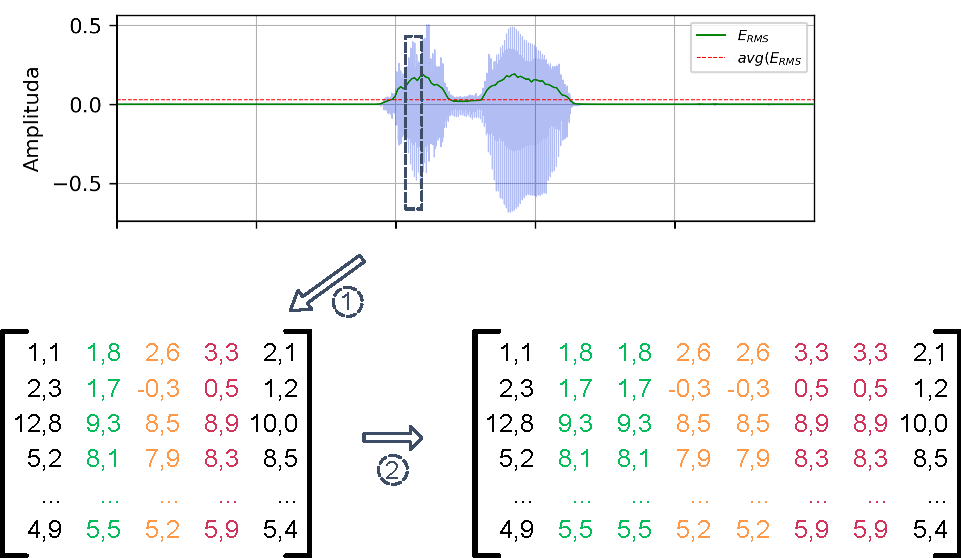
\includegraphics[width=0.9\textwidth]{./ch4-experiments/img/augmentation_features.pdf}
  \caption{Princip protažení na příznacích.}
  \label{fig:experiments:augmentation:features}
\end{figure}

Protažení na příznacích je, ale spíše hypotetická možnost. V reálné situaci by totiž řečník mluvil jako doposud a k protažení by docházelo při zpracování. Což je velmi netriviální úkol. Teoreticky by se musel v rámci parametrizace doplnit mechanismus, který by určité příznakové vektory určitým způsobem duplikoval. Navíc prosté zkopírování porušuje dynamický charakter řeči. V rámci jednoho zpracovávaného okénka (jednoho vektoru) jsou parametry považovány za statické, ale jak se okénko v rámci zpracování posouvá, tak už nelze hovořit o stacionaritě parametrů. Tento problém by se musel řešit nějakým druhem interpolace mezi dvěma konsekutivními vektory. Mechanismus by zároveň vyřešil omezení, kdy je kopírováním možné získat pouze protažení odpovídající celočíselnému násobku původní délky. Proč tedy vůbec zkoušet tento typ protažení? Odpověď je jednoduchá, nehraje zde takovou roli přesnost zarovnání. V průběhu zpracování je využíváno posuvného okénka a překryvu. Díky tomu dojde k určitému \uv{rozmazání} hranic. Pro úplně prvotní experimenty je to pak relativně vítané zjednodušení úlohy.

\subsubsection{Dosažené výsledky}

Prvním bodem výše zmíněného algoritmu je získání standardního modelu, který je použit k zarovnání dat. K tomu je možné použít již natrénovaný model z části \ref{chap:experiments:normalization:quality}. Jde tedy o \textit{HMM-DNN} model s $5$ skrytými vrstvami, každá s $4096$ neurony. Výstupní vrstva je pak typu softmax dimenze rovné počtu HMM stavů. Tento model dosáhl s monofónovým zerogramovým LM přesnoti $84,66\ \%$. S jeho pomocí je získáno zarovnání, tedy hranice jednotlivých fónému v trénovací i testovací sadě. Díky zarovnání je možné protáhnout zájmové fonémy.

V rámci testování celého procesu je jako prvotní ověřovací experiment zvoleno dvojnásoné protažení fonému $/s/$. Jinými slovy, všechny vektory odpovídající $/s/$ jsou zduplikovány. Následně je standardním způsobem natrénován \textit{HMM-DNN} model. Neuronová síť má tedy $5$ skrytých vrstev s $4096$. Výstupní vrstva je typu softmax. Otestování je pak jako v předchozích případech realizováno na testovací sadě s monofónovým zerogramovým jazykovým modelem. Tento nový model dosáhl přesnosti $85,11\ \%$, což je sice malé, ale přesto zlepšení.

Protažení $/s/$ posloužilo hlavně k ověření procesu vytváření modelu. Další experiment je realizován na protažených fonémech $/k/$, $/p/$, $/s/$, $/t/$ a $/v/$, což představuje většinu neznělých zájmových fonémů. Zarovnání je identické jako u předchozího experimentu, protože původní data se nezměnila. Opět je uvažováno dvojnásobné protažení. Všechny vektory inkriminovaných fonémů jsou zduplikovány. Znovu je natrénován \textit{HMM-DNN} model a otestován společně s monofonovým zerogramovým jazykovým modelem. Přesnost na testovací sadě dosáhla hodnoty $87,50\ \%$, což lze považovat za významné zlepšení.

Doposud se uvažovalo pouze o dvojnásobném protažení, v další fázi je tedy potřeba oveřit jestli jiné hodnoty nemohou poskytnout ještě lepší výsledek. Celkem je uvožované $3x$, $4x$ a $5x$ protažení. Uvažovány jsou fonémy $/k/$, $/p/$, $/s/$, $/t/$ a $/v/$. Proces natrénování a otestování modelu je stejný jako v předchozích případech. Dosažené výsledky jsou pak v tab. \ref{tab:experiments:augmentation:influence}. Pro úplnost je tabulka doplněna o baseline model s $1x$ protažením (tedy žádným) a již prezentované $2x$ protažení. Z výsledků je patrný jasný trend, větší než $2x$ protažení nemá smysl, protože se přesnost zhoršuje. Optimální hodnota protažení teoreticky leží někde v intervalu $\left(1,\ 3\right)x$, ale s protahovaním pomocí kopírování příznakových vektorů není možné přesné určení hodnoty.

\begin{table}[htpb]
  \centering
  \def\arraystretch{1.5}
  \pgfplotstabletypeset[
    col sep=semicolon,
    string type,
    columns/extension/.style={column name=, column type={|l}},
    columns/1x/.style={column name=1x, column type={|r}},
    columns/2x/.style={column name=2x, column type={|r}},
    columns/3x/.style={column name=3x, column type={|r}},
    columns/4x/.style={column name=4x, column type={|r}},
    columns/5x/.style={column name=5x, column type={|r|}},
    every head row/.style={after row=\hline, before row=\hline},
    every last row/.style={after row=\hline},
  ]{./ch4-experiments/tabs/0301-features.csv}
  \caption{Vliv míry protažení na přesnost modelu.}
  \label{tab:experiments:augmentation:influence}
\end{table}

Zhoršení přesnosti dozajista souvísí s faktem, že výsledná augmentovaná data neodpovídají realitě. Čím vícekrat je vektor zkopírován, tím více je vnášena chyba způsobená ignorováním dynamické povahy signálu. Nicméně jako proof-of-concept myšlenky posloužil tento experiment velmi dobře. Protažení na příznacích vede ke zvýšení přesnosti a má smysl tuto cestu více prozkoumat.

\subsection{Protažení na zvuku}
\label{chap:experiments:augmentation:audio}

Protažení na příznacích vedlo ke významnému zlepšení, ale tento přístup není bohužel reálně použitelný. Tím může být až model pracující s fonémy protaženými přímo v audiu. Tato data budou totiž mnohem více odpovídat případným reálným datům získaným od řečníka.

Stejně jako v předchozím případě je k protažení potřeba zarovnání. To s určitou mírou přesnosti určuje počáteční a koncové hranice jednotlivých fonémů. Na základě je možné určitý úsek protáhnout například pomocí:

\begin{itemize}
  \item převzorkování signálu,
  \item TD-PSOLA algoritmu,
  \item fázového vokodéru.
\end{itemize}

\noindent Asi nejednodušší je převzorkování dat, stačí načíst všechny vzorky odpovídající vybranému fonému a změnit vzorkovací frekcenci. Pokud je cílem úsek protáhnout, tak je výsledná nová vzorkovací frekvence menší než originální. Hlavním problémem této metody je tonální posun\footnote{Mění se fundamentální frekvence $F_0$. Pokud došlo ke zrychlení, tak je vyšší. Při zpomalení naopak nižší.}. Cílem je protáhnout jeden foném, který z celkové délky nahrávky zabírá jen malou část, a proto by se dal tento nepříznivý jev ignorovat. Snaha je však vygenerovat co možná nejreálnější protažené nahrávky, a proto není protažení pomocí převzorkování nejvhodnější metodou.

Zbylé dva uvažované přístupy umožňují sofistikovanější úpravy signálu. Snahou je upravit časové vlastnosti signálu aniž by byl nepříznivě ovlivněn tón.  Obě metody využívají \textit{analýzy} signálu,  následováné \textit{zpracováním} a zakončené \textit{syntézou}. Rozdíl je hlavně ve způsobu. Metody z rodiny \textit{PSOLA} pracují s hlasivkovými pulsy, které jsou nejprve v analytické části nalezeny\footnote{Výsledkem analýzy jsou periodicky se opakující značky, angl. pitch marks. Úpravou jejich parametrů dochází ke změnám parametrů řeči.}, aby pak v části zpracování došlo k jejich transformaci na základě požadavků na výslednou řeč. V posledním kroku dochází k syntéze signálu na základě upravených analytických krátkodobých signálů, tedy hlasivkových pulsů. Více detailnějí se o této metodě hovoří v \cite{Psutka2006}.

Fázový vokodér pracuje na podobném principu, s tím rozdílem, že v analytické části dochází k převodu signálu do frekveční oblasti pomocí FFT. Ve fázi zpracování je potom signál upraven, aby ve fázi syntézy byl opět převeden do časové oblasti pomocí inverzní FFT.

Pomocí těchto dvou zmíněných metod je možné upravit nejen délku, ale i $F_0$ signálu. Stejně jako u převzorkování mají neblahý vliv na signál, ale ten není tak výrazný jako v případě převzorkování. U \textit{TD-PSOLA} mohou například vznikat artefakty způsobnené nespojitostmi mezi sousedními upravenými úseky řeči. U fázového vokodér nevznikají artefakty vlivem nespojitostí, ale vlivem fázového posunu. Jelikož se signál upravuje ve frekveční oblasti, kde dochází ke změnám jednotlivých komponent, může dojít k fázovému posunu mezi jednotlivými komponentami. Při syntéze pak mohou vznikat zaznamenatelné artefakty připomínající tupý zvuk.

Obě metody však poskytují velmi dobré výsledky protažená na jednotlivých fonémech. Výsledné protažení je téměř identické. Interně vyvinutý nástroj umožňující ovlivnění délky řeči (a priory používaný při syntéze řeči) poskytuje obě sofistikované metody. Pro výsledné protažení je pak použita metoda \textit{TD-PSOLA}. Ukázka původního a protaženého slova \uv{kosa} je pak na obr. \ref{fig:experiments:augmentation:compare}. Protahován byl foném $/s/$, který je v signálu vidět jako šum mezi dvěmi výraznými častmi signálu. Inkriminovaný foném byl protažen na přibližně dvojnásobek. Na obr. \ref{fig:experiments:augmentation:compare:augmented} je pak zřetelně vidět protažení úseku odpovídající $/s/$. Zároveň v signálu a ani ve spektru není vidět, žádný významný artefakt.

\begin{figure}[htpb]
  \centering
  \begin{subfigure}[b]{0.42\textwidth}
    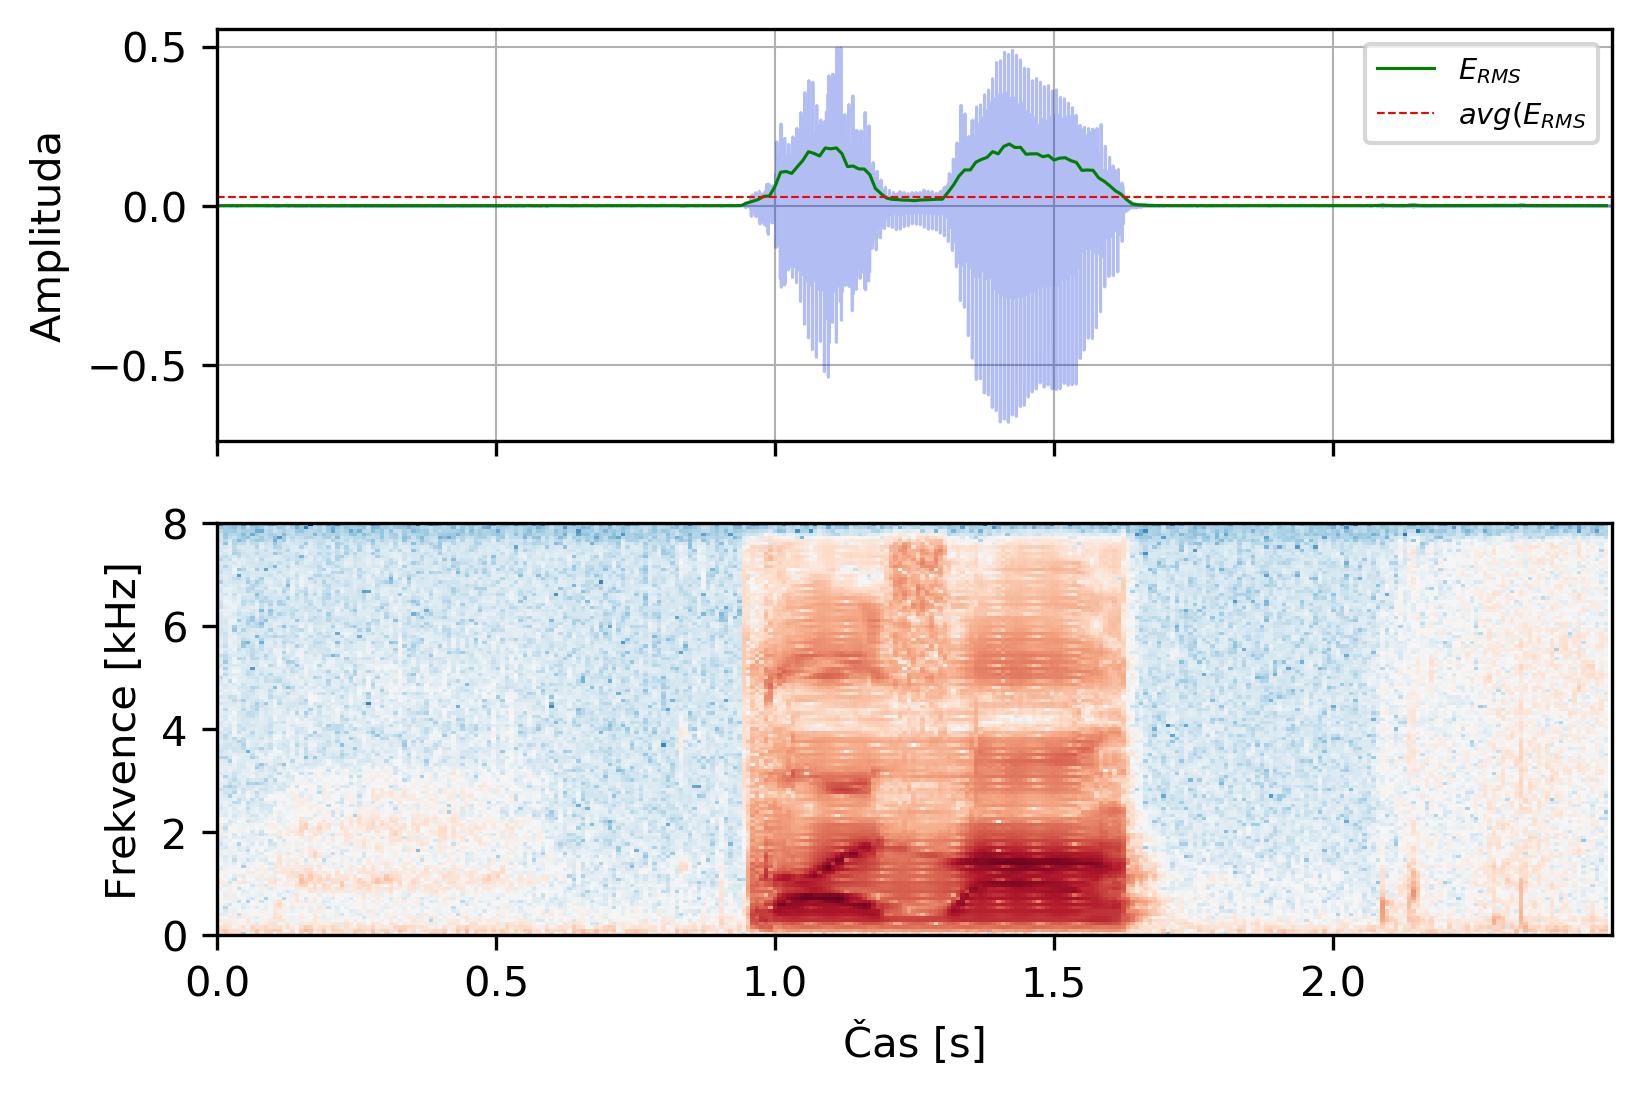
\includegraphics[width=\textwidth]{./ch4-experiments/img/energy_spec_word-normal.png}
    \caption{Originální}
    \label{fig:experiments:augmentation:compare:original}
  \end{subfigure}
  %
  \begin{subfigure}[b]{0.42\textwidth}
    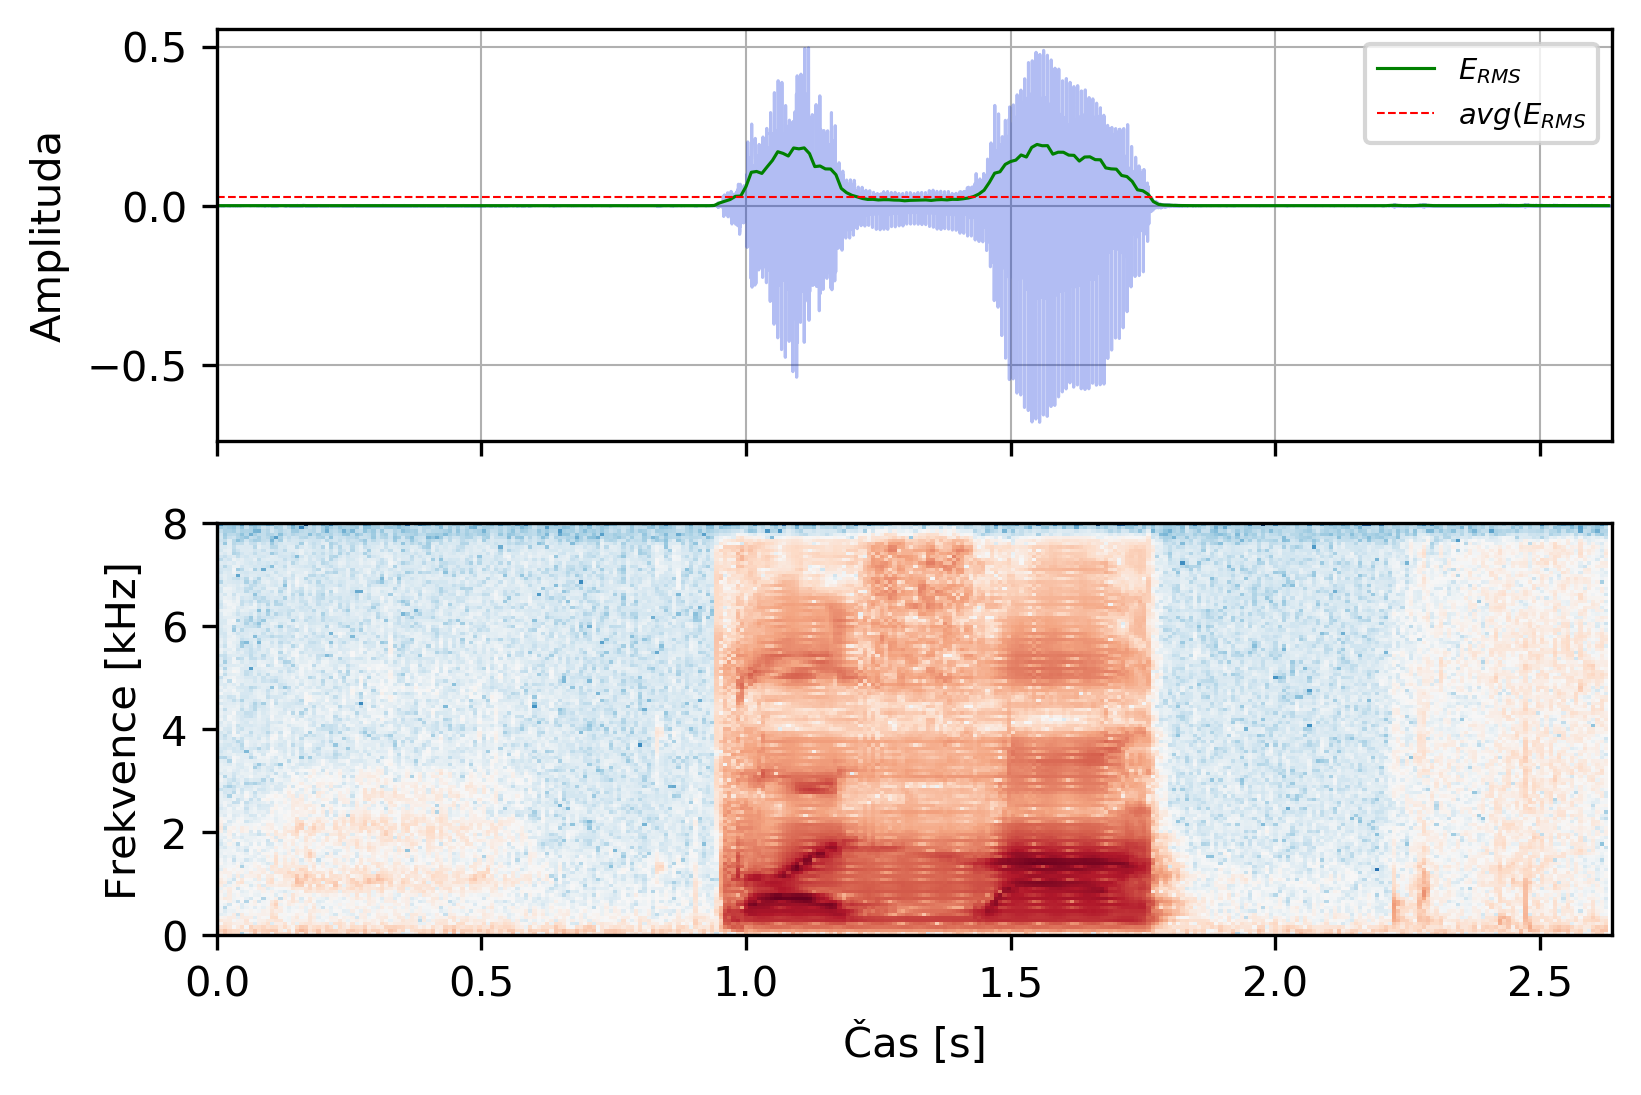
\includegraphics[width=\textwidth]{./ch4-experiments/img/energy_spec_word-augmented.png}
    \caption{Protažené}
    \label{fig:experiments:augmentation:compare:augmented}
  \end{subfigure}
  \caption{Amplituda a spektrogram původního (protaženého) slova \uv{kosa}.}
  \label{fig:experiments:augmentation:compare}
\end{figure}

\subsubsection{Dosažené výsledky s DNN}

K ověření schopností modelu pracovat s uměle protaženými daty je použit stejný \textit{HMM-DNN} model jako v předchozích případech. Neuronová síť má $5$ skrytých vrstev, každá s $4096$ neurony. Výstupní vrstva je pak typu softmax dimenze rovné počtu HMM stavů. V datech jsou protaženy všechny výskyty fonémů $/k/$, $/p/$, $/s/$, $/t/$ a $/v/$. Uvažováno je protažení $1,25x$, $1,50x$, $1,75x$ a $2,00x$. Jazykový model je stejně jako v případě protažení na příznacích monofónový zerogramový. Dosažené výsledky jsou vypsány v tab. \ref{tab:experiments:augmentation:influence:dnn}. Nejlepšího výsledku dosáhl \textit{baseline} model s hodnotou $84,66\ \%$. S libovolným protažením dochází k poklesu přesnosti, což je nepochyně zklamáním.

\begin{table}[htpb]
  \centering
  \def\arraystretch{1.5}
  \pgfplotstabletypeset[
    col sep=semicolon,
    string type,
    columns/extension/.style={column name=, column type={|l}},
    columns/100/.style={column name={1,00x}, column type={|r}},
    columns/125/.style={column name={1,25x}, column type={|r}},
    columns/150/.style={column name={1,50x}, column type={|r}},
    columns/175/.style={column name={1,75x}, column type={|r}},
    columns/200/.style={column name={2,00x}, column type={|r|}},
    every head row/.style={after row=\hline, before row=\hline},
    every last row/.style={after row=\hline},
  ]{./ch4-experiments/tabs/0302-audio_1.csv}
  \caption{Vliv míry protažení fonému na přesnost DNN modelu.}
  \label{tab:experiments:augmentation:influence:dnn}
\end{table}

\subsubsection{Upravené zarovnání a time delay neural network}

Při analýze výsledků se ukázalo, že zarovnání v mnoha případech není zrovna nejpřesnější a to zvláště u inkriminovaných neznělých fonémů. Na obr. \ref{fig:experiments:augmentation:alignemnt:wrong} je získané zarovnání slova \uv{kosa} a také vyznačené hranice v audiu a spektru. Z obr. \ref{fig:experiments:augmentation:alignemnt:wrong:audio} je zřejmé, že počáteční hranice $/s/$ zasahuje ještě do předchozího fonému $/o/$. Tím pádem dochází k protažení nevhodné části signálu a model se tak učí na špatných datech. Pokud by samozřejmě všechny fonémy $/s/$ následovaly po $/o/$, tak by to víceméně nebyl problém, ale to samozřejmě neplatí.

\begin{figure}[htpb]
  \centering
  \begin{subfigure}[b]{0.26\textwidth}
    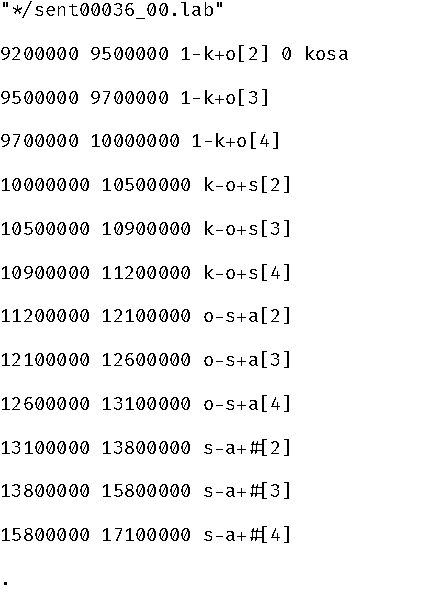
\includegraphics[width=\textwidth]{./ch4-experiments/img/alignment_text.pdf}
    \caption{Zarovnání}
    \label{fig:experiments:augmentation:alignemnt:wrong:text}
  \end{subfigure}
  %
  \begin{subfigure}[b]{0.55\textwidth}
    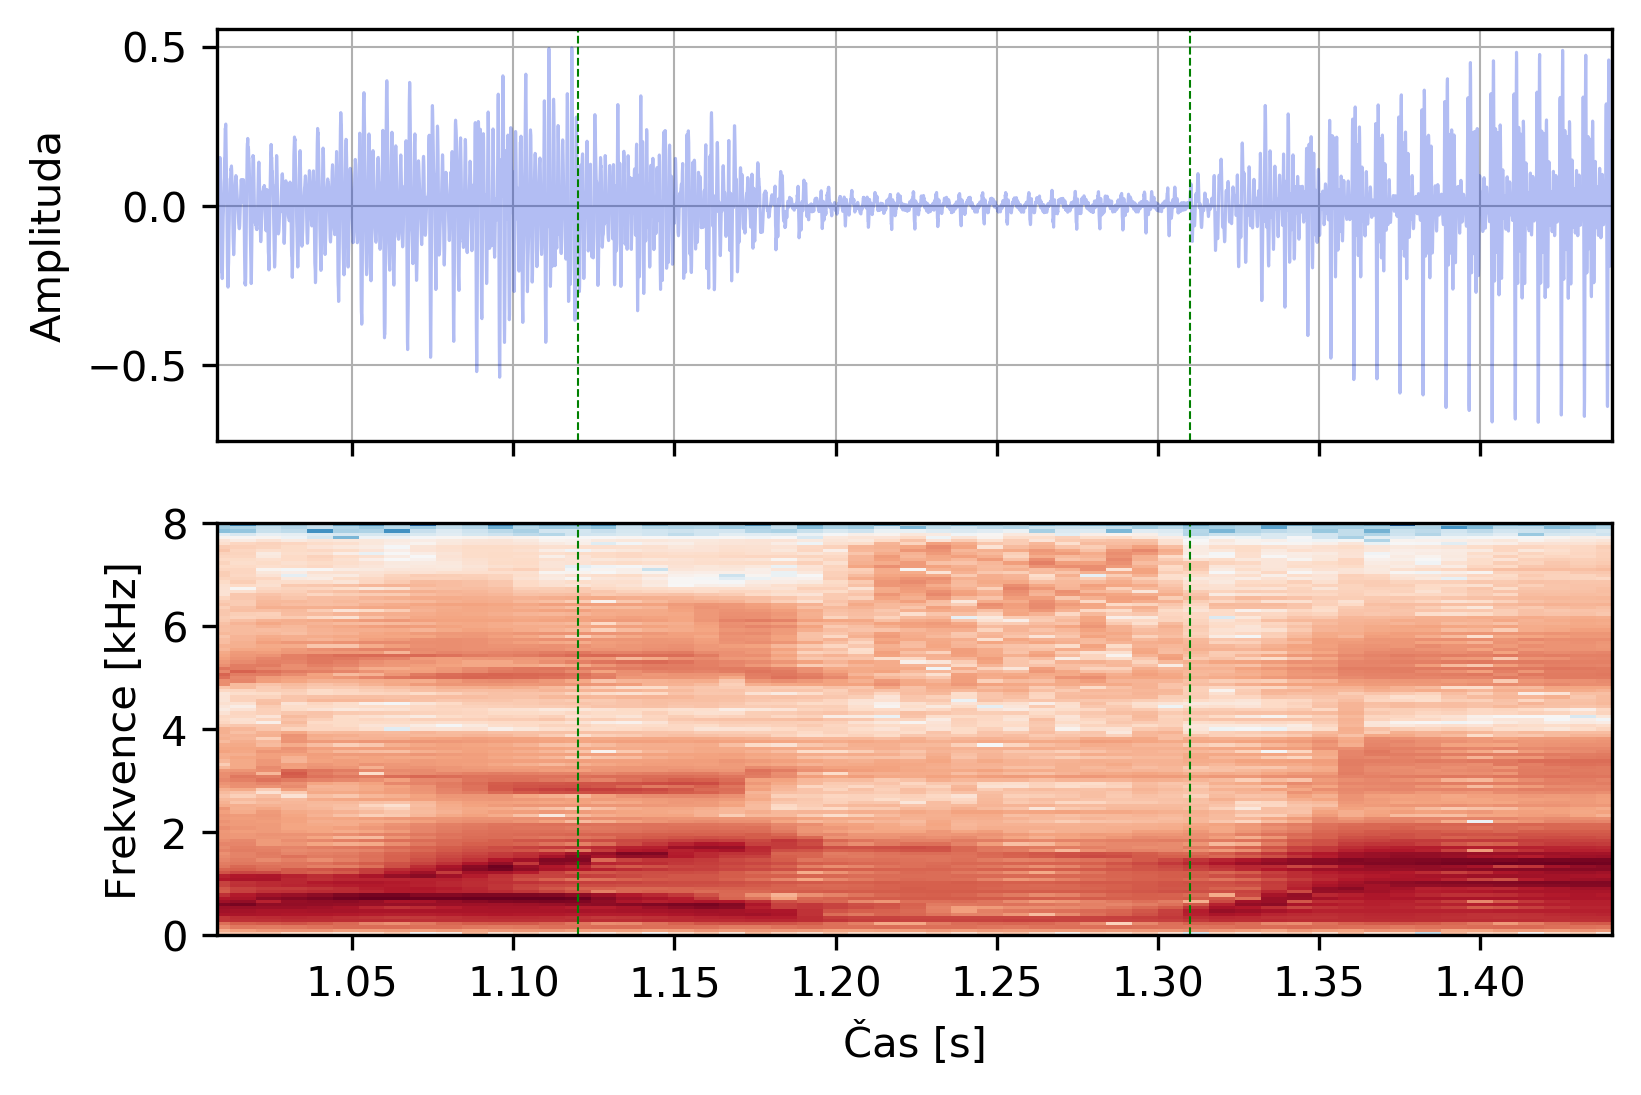
\includegraphics[width=\textwidth]{./ch4-experiments/img/energy_spec_word-segment.png}
    \caption{V signálu}
    \label{fig:experiments:augmentation:alignemnt:wrong:audio}
  \end{subfigure}
  \caption{Špatně zarovnaný foném $/s/$ ve slově \uv{kosa}.}
  \label{fig:experiments:augmentation:alignemnt:wrong}
\end{figure}

%Pro lepší zarovnání je potřeba upravit model, který se o zarovnání stará. \todo{TBD}{Doplnit vysvětlení od Pepika.}

V době experimentů s protažením konkrétních fonémů se začaly stále více prosazovat time delay neural networks (TDNN). Přestože patří do rodiny feed-forward sítí jako DNN, tak se oproti nim snaží vzít v potaz i dynamickou složku řeči\footnote{DNN berou v úvahu pouze statické vlastnosti řeči, protože síť v každém okamžiku zpracovává vektor příznaků odpovídající určitému času $t_c$ a jeho okolí. V čase $t_{c+1}$ není nijak zohledněn předchozí výsledek v čase $t_c$.}. U DNN jsou všechny neurony v jednotlivých vrstvách propojeny a tedy vstupní vektor je zpracováván všemi neurony v následující vrstvě. U TDNN toto neplatí, neurony v určité vrtvě jsou propojeny vždy jen s určitým počtem neuronů ve vrstvě následující, viz obr. \ref{fig:experiments:augmentation:tdnn}. To v důsledku znamená, že části sítě vykonávájí rozhodnutí na základě jiných podmnožin vstupních dat. V dalších vrstvách se pak tyto lokální rozhodnotí integrují, aby na výstupu sítě došlo ke globálnímu rozhodnutí. Tedy, aby byl výstupem sítě foném odpovídající času $t_c$ a jeho okolí $\langle t_{c-n}; t_{c+m} \rangle$.

S posunem okénka velikosti $m + n + 1$ postupně jednotlivé části sítě zpracují všechny části vstupního zparametrizovaného signálu. Dynamika je zohledněna další množinou vah, která se mění podle toho jakou část vstupního vektoru ta část sítě zpracovává \cite{Waibel1989}. Tento přístup by se dal přirovnat k konvoluční neuronové síti (CNN), kde se také vstupní data (většinou obrázky) nezpracovájí najednou, ale pomocí filtrů vždy jen malá podmnožina. A v dalších vrstvách dochází ke spojování výsledků z těchto podmnožin. Hlavní rozdíl mezi TDNN a CMN je v tom, že CMN nepracuje s konceptem času. Více množin vah lze považovat za určitý ekvivalent paměti u RNN sítí.

\begin{figure}[hbpt]
  \centering
  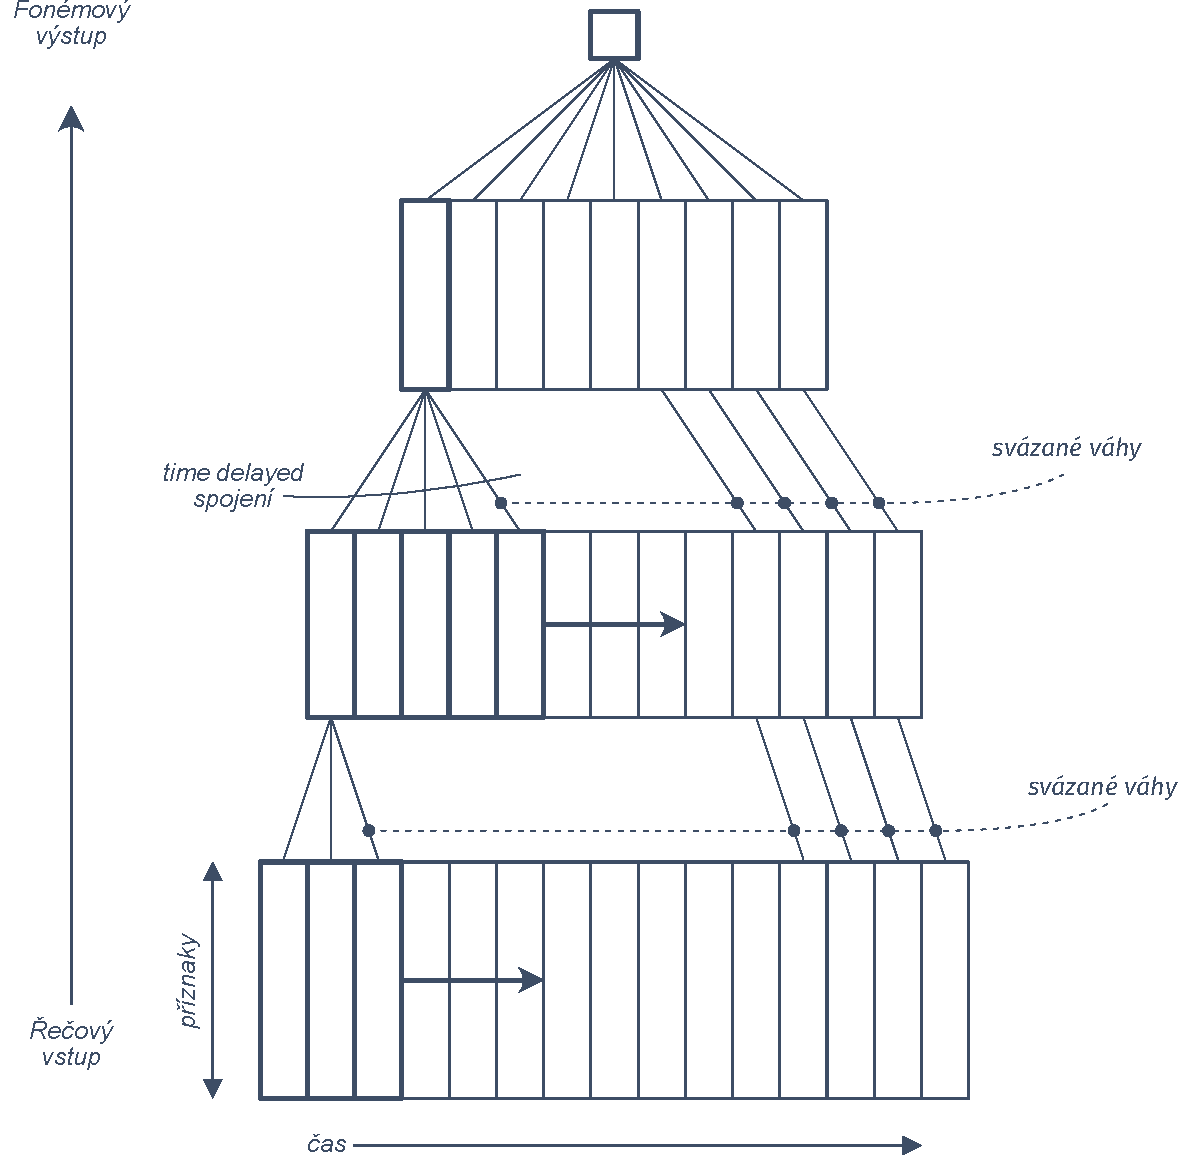
\includegraphics[width=0.5\textwidth]{./ch4-experiments/img/tdnn.pdf}
  \caption{Time delay neural network (TDNN).}
  \label{fig:experiments:augmentation:tdnn}
\end{figure}

Stejně jako u DNN je na počátku trénování nutné mít k dispozici zarovnání. To, ale nemusí být naprosto přesné, protože je vstupní vektor zpracováván jiným způsobem než u DNN a pomocí více množin vah je brán v potaz i dynamický charakter řeči \cite{Peddinti2015}. Model založený na TDNN by tak měl ve výsledku generovat přesnější zarovnání a tím zlepšit výsledky modelu pracující s uměle protaženými daty.

Jako startovní bod trénování je použito DNN zarovnání z předchozího experimentu. Topologie sítě vychází z hodnot prezentovaných v \cite{Peddinti2015}, tedy síť má $4$ skryte vrstvy. Velikost jednotlivých vrstev závisí na uvažovaném kontextu v jednotlivých vrstvách. První vrstava uvažuje kontext $m=2$ a $n=2$, ostatní vrstvy pak odpovídají nejlepší sítí z \cite{Peddinti2015}. Ukázka zarovnání získané touto sítí je znázorněna na obr. \ref{fig:experiments:augmentation:alignemnt:correct}. Z vyznačených hranic fonému $/s/$ (obr. \ref{fig:experiments:augmentation:alignemnt:correct:audio}) ,ve slově \uv{kosa}, je patrné v podstatě přesné určení počáteční a koncové hranice fonému. Lepší zarovnání naznačuje i lepší vlastnosti modelu. Pro ověření této hypotézy opět poslouží standardní experiment s monofonovým zerogramovým LM, v něm TDNN síť dosáhla přesnosti $85,41$. Síť tedy dosáhla nepatrně lepšího výsledku než DNN síť.

\begin{figure}[htpb]
  \centering
  \begin{subfigure}[b]{0.26\textwidth}
    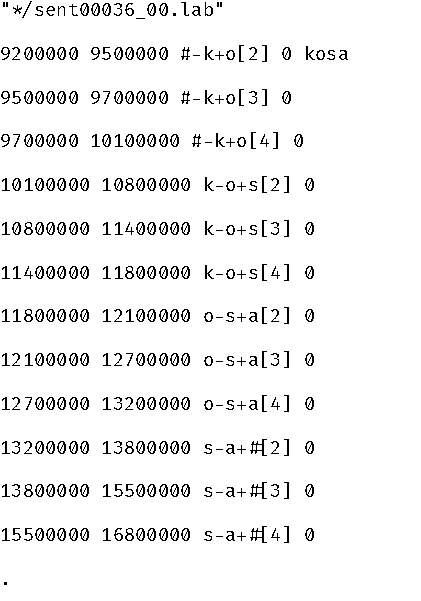
\includegraphics[width=\textwidth]{./ch4-experiments/img/alignment_text-2.pdf}
    \caption{Zarovnání}
    \label{fig:experiments:augmentation:alignemnt:correct:text}
  \end{subfigure}
  %
  \begin{subfigure}[b]{0.55\textwidth}
    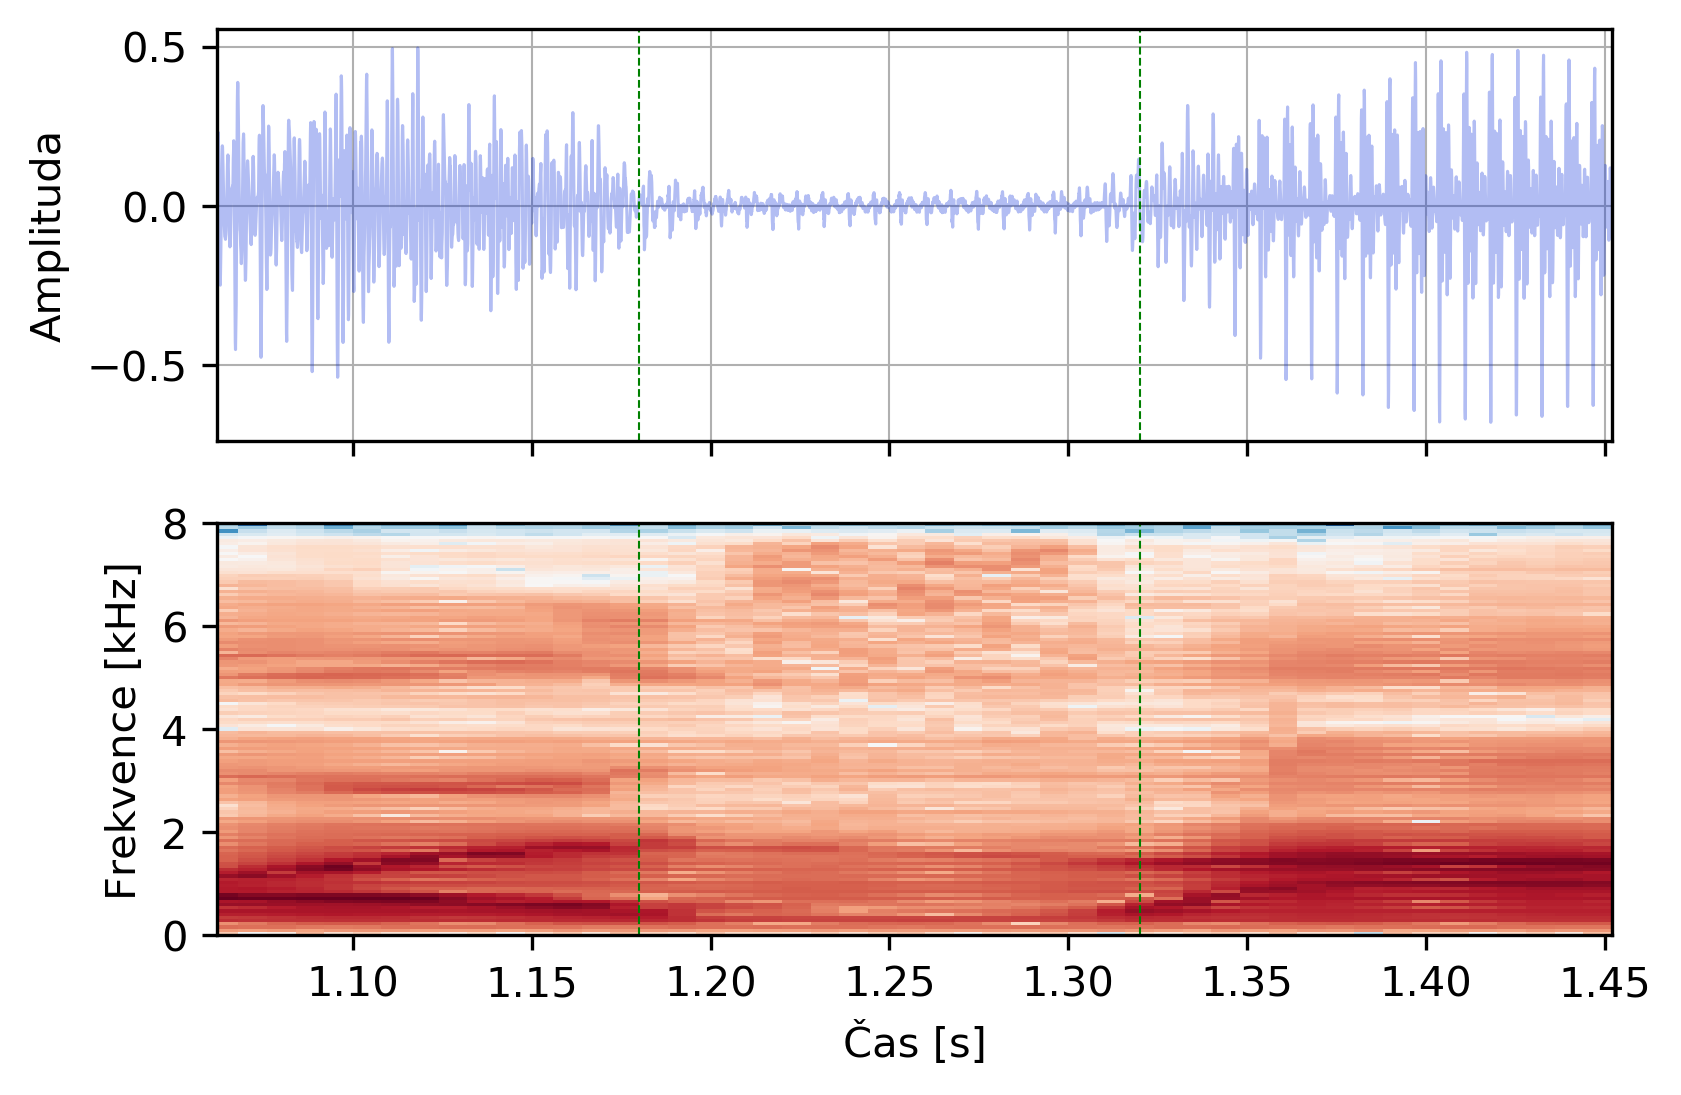
\includegraphics[width=\textwidth]{./ch4-experiments/img/energy_spec_word-segment-2.png}
    \caption{V signálu}
    \label{fig:experiments:augmentation:alignemnt:correct:audio}
  \end{subfigure}
  \caption{Správně zarovnaný foném $/s/$ ve slově \uv{kosa}.}
  \label{fig:experiments:augmentation:alignemnt:correct}
\end{figure}

Poté co je k dispozici relativně přesné zarovnání, je možné přistoupit k protažení fonémů $/k/$, $/p/$, $/s/$, $/t/$ a $/v/$ a natrénování modelu pracující s těmito daty. Na začátku je nutné natrénovat \textit{HMM-GMM} model, který poskytne prvotní zarovnání. V předchozích experimentech následovalo natrénování DNN modelu, ale aplikace TDNN na zarovnání ukázala lepší vlastnosti tohoto modelu. Jako další model je tedy natrénována TDNN síť. K otestování modelu je použit standarní monofónový zerogramová jazykový model. Uvažováno je protažení $1,25x$ do $3,00x$ s krokem $0,25$. Výsledky experimentu jsou pak vypsány v tab. \ref{tab:experiments:augmentation:influence:tdnn}. Oproti výsledkům v tab. \ref{tab:experiments:augmentation:influence:dnn} je vidět výrazné zlepšení přesnoti modelu oproti baselinu s $85,41\ \%$. Nejvyšší přesnosti $87,90\ \%$ dosáhl model pracující s $2,5x$ protaženými daty. Navíc modely pracující s protažením od $1,75x$ do $2,75x$ dosahují velmi podovných výsledků, což poskytuje relativně široký pracovní interval pro případné skutečně protažená data řečníkem.

\begin{table}[htpb]
  \centering
  \def\arraystretch{1.5}
  \pgfplotstabletypeset[
    col sep=semicolon,
    string type,
    columns/extension/.style={column name=, column type={|l}},
    columns/100/.style={column name={1,00x}, column type={|r}},
    columns/150/.style={column name={1,50x}, column type={|r}},
    columns/125/.style={column name={1,25x}, column type={|r}},
    columns/175/.style={column name={1,75x}, column type={|r}},
    columns/200/.style={column name={2,00x}, column type={|r}},
    columns/225/.style={column name={2,25x}, column type={|r}},
    columns/250/.style={column name={2,50x}, column type={|r}},
    columns/275/.style={column name={2,75x}, column type={|r}},
    columns/300/.style={column name={3,00x}, column type={|r|}},
    every head row/.style={after row=\hline, before row=\hline},
    every last row/.style={after row=\hline},
  ]{./ch4-experiments/tabs/0303-audio_2.csv}
  \caption{Vliv míry protažení fonému na přesnost TDNN modelu.}
  \label{tab:experiments:augmentation:influence:tdnn}
\end{table}

\subsection{Reálně protažená data}
\label{chap:experiments:augmentation:real}

\begin{itemize}
  \item problém se znělostí (systém moc nefunguje pokud je promluva krátká)
  \item popsat důvody pro protažení
  \item popis a výsledky experimentů na uměle protažených datech na příznacích (není použitelné reálně)
  \item aktualizace experimentu \uv{člověk vs. stroj}
\end{itemize}
